%%%%%%%%%%%%%%%%%%%%%%%%%%%%%%%%%%%%%%%%%
% Beamer Presentation
% LaTeX Template
% Version 1.0 (10/11/12)
%
% This template has been downloaded from:
% http://www.LaTeXTemplates.com
%
% License:
% CC BY-NC-SA 3.0 (http://creativecommons.org/licenses/by-nc-sa/3.0/)
%
%%%%%%%%%%%%%%%%%%%%%%%%%%%%%%%%%%%%%%%%%

%----------------------------------------------------------------------------------------
%	PACKAGES AND THEMES
%----------------------------------------------------------------------------------------

\documentclass{beamer}

\mode<presentation> {

% The Beamer class comes with a number of default slide themes
% which change the colors and layouts of slides. Below this is a list
% of all the themes, uncomment each in turn to see what they look like.

\usetheme{default}
%\usetheme{AnnArbor}
%\usetheme{Antibes}
%\usetheme{Bergen}
%\usetheme{Berkeley}
%\usetheme{Berlin}
%\usetheme{Boadilla}
%\usetheme{CambridgeUS}
%\usetheme{Copenhagen}
%\usetheme{Darmstadt}
%\usetheme{Dresden}
%\usetheme{Frankfurt}
%\usetheme{Goettingen}
%\usetheme{Hannover}
%\usetheme{Ilmenau}
%\usetheme{JuanLesPins}
%\usetheme{Luebeck}
%\usetheme{Madrid}
%\usetheme{Malmoe}
%\usetheme{Marburg}
%\usetheme{Montpellier}
%\usetheme{PaloAlto}
%\usetheme{Pittsburgh}
%\usetheme{Rochester}
%\usetheme{Singapore}
%\usetheme{Szeged}
%\usetheme{Warsaw}

% As well as themes, the Beamer class has a number of color themes
% for any slide theme. Uncomment each of these in turn to see how it
% changes the colors of your current slide theme.

%\usecolortheme{albatross}
%\usecolortheme{beaver}
%\usecolortheme{beetle}
%\usecolortheme{crane}
%\usecolortheme{dolphin}
%\usecolortheme{dove}
%\usecolortheme{fly}
%\usecolortheme{lily}
%\usecolortheme{orchid}
%\usecolortheme{rose}
%\usecolortheme{seagull}
\usecolortheme{seahorse}
%\usecolortheme{whale}
%\usecolortheme{wolverine}

%\setbeamertemplate{footline} % To remove the footer line in all slides uncomment this line
\setbeamertemplate{footline}[page number] % To replace the footer line in all slides with a simple slide count uncomment this line

\setbeamertemplate{navigation symbols}{} % To remove the navigation symbols from the bottom of all slides uncomment this line
}

%\setbeamertemplate{headline} 

\usepackage{graphicx} % Allows including images
\usepackage{booktabs} % Allows the use of \toprule, \midrule and \bottomrule in tables
\usepackage[export]{adjustbox}
\usepackage{amsmath}
\usepackage[utf8]{inputenc}
\usepackage{setspace}

%----------------------------------------------------------------------------------------
%	TITLE PAGE
%----------------------------------------------------------------------------------------
%Unfolding the Quantitative Dynamics of Biological Networks
\title[George Christodoulis]{Diploma Thesis: Communication Modeling and Placement of Parallel Applications} % The short title appears at the bottom of every slide, the full title is only on the title page
\subtitle{{\fontsize{8}{6}\selectfont Supervisors: Nektarios Kozyris (CSLab/ECE/NTUA), Georgios Goumas (CSLAB/ECE/NTUA)}}
\author{Georgios Christodoulis} % Your name
\institute[NTUA] % Your institution as it will appear on the bottom of every slide, may be shorthand to save space
{
ECE$-$NTUA \\ % Your institution for the title page
\medskip
\textit{gchristodoulis@gmail.com} % Your email address
}
\date{}

\begin{document}

\begin{frame}
\titlepage % Print the title page as the first slide
\end{frame}

%%%%%%%%%%%%%%%%%%%%%%%%%%%%%%%%%%%%%%%%%%%%%%%%%%%%%%%%%%%%%%
%			Uncomment for Overview..not for now
%%%%%%%%%%%%%%%%%%%%%%%%%%%%%%%%%%%%%%%%%%%%%%%%%%%%%%%%%%%%%%
%\begin{frame}
%\frametitle{Overview} % Table of contents slide, comment this block out to remove it
%\tableofcontents % Throughout your presentation, if you choose to use \section{} and \subsection{} commands, 
%these will automatically be printed on this slide as an overview of your presentation
%\end{frame}
%%%%%%%%%%%%%%%%%%%%%%%%%%%%%%%%%%%%%%%%%%%%%%%%%%%%%%%%%%%%%%
%----------------------------------------------------------------------------------------
%	PRESENTATION SLIDES
%----------------------------------------------------------------------------------------
%------------------------------------------------

\begin{frame}
\frametitle{Parallel Architectures}
\begin{columns}[c]

\column{.8\textwidth}
\linespread{0.5}
\begin{block}{Shared Memory}
\begin{enumerate}
\item {\fontsize{8}{6}\selectfont Processors share the same physical memory}
\item {\fontsize{8}{6}\selectfont Local cache memory hierarchy}
\item {\fontsize{8}{6}\selectfont Connection via memory bus}
\end{enumerate}
\end{block}

\begin{block}{Distributed Memory}
\begin{enumerate}
\item {\fontsize{8}{6}\selectfont Every processor has its own memory hierarcy}
\item {\fontsize{8}{6}\selectfont Processor communication via interconnection network}
\end{enumerate}
\end{block}

\begin{block}{Hybrid Architectures}
Dominant architecture for modern supercomputers.
\end{block}

\column{.3\textwidth}
\begin{figure}
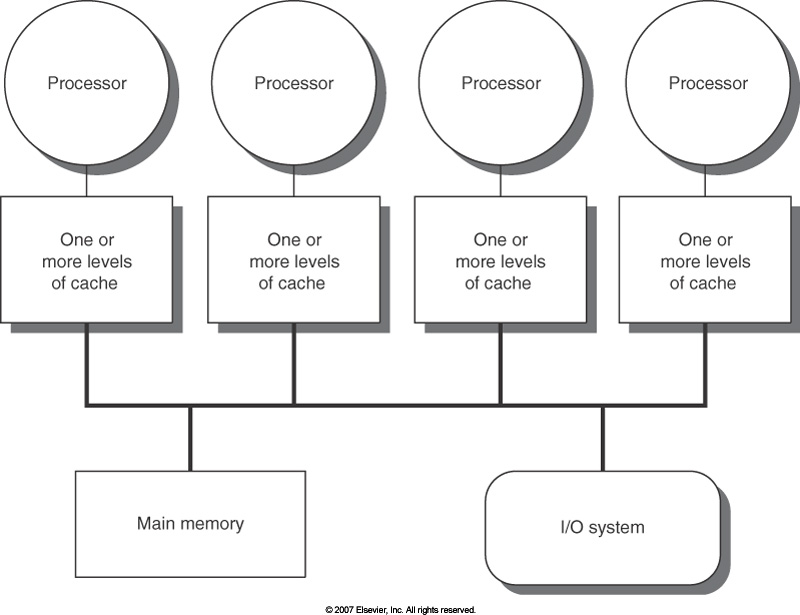
\includegraphics[width=\linewidth,right]{shared_mem.jpg}
\end{figure}

\begin{figure}
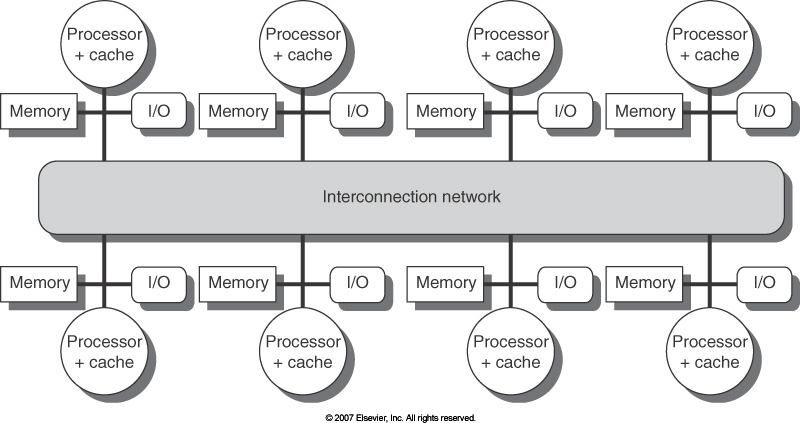
\includegraphics[width=\linewidth,right]{distributed_mem.jpg}
\end{figure}

\begin{figure}
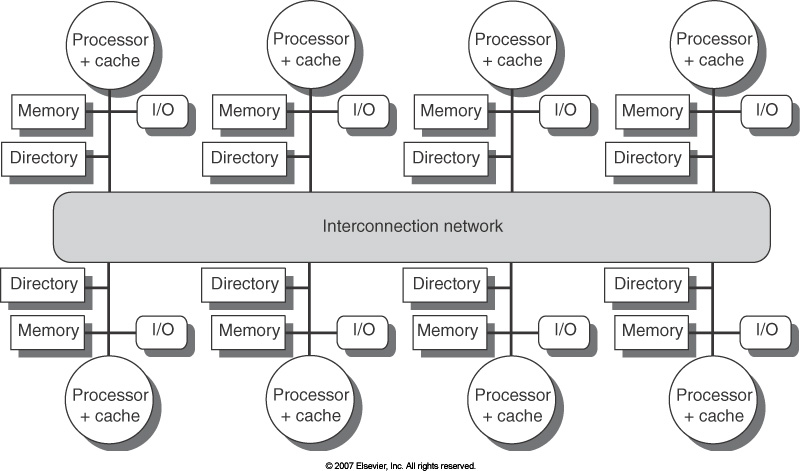
\includegraphics[width=\linewidth,right]{hybrid_mem.jpg}
\end{figure}

\end{columns}

\end{frame}
%------------------------------------------------

\begin{frame}
\frametitle{Parallel Programming Models}
\begin{columns}[c]

\column{.8\textwidth}
\linespread{0.5}
\begin{block}{OpenMP - Shared Memory Model}
\begin{enumerate}
\item {\fontsize{8}{6}\selectfont Compiler directives based tools}
\item {\fontsize{8}{6}\selectfont Suitable for shared memory architectures}
\item {\fontsize{8}{6}\selectfont Popular Schemas: Fork/Join, SPMD, parallel for, Master/Workers}
\end{enumerate}
\end{block}

\begin{block}{MPI - Distributed Memory Model}
\begin{enumerate}
\item {\fontsize{8}{6}\selectfont Message Passing Library}
\item {\fontsize{8}{6}\selectfont SPMD - Every process runs the same program}
\item {\fontsize{8}{6}\selectfont Collective vs P2P}
\item {\fontsize{8}{6}\selectfont Blocking vs non-Blocking}
\end{enumerate}
\end{block}

\begin{block}{OpenMP/MPI-Hybrid Model}
\begin{enumerate}
\item {\fontsize{8}{6}\selectfont Best fit for Hybrid architectures}
\item {\fontsize{8}{6}\selectfont OpenMP - intranode communication }
\item {\fontsize{8}{6}\selectfont MPI - communication through the interconnection network}
\end{enumerate}
\end{block}

\column{.01\textwidth}

\end{columns}

\end{frame}
%------------------------------------------------

\begin{frame}
\frametitle{Our System}

\begin{columns}[c]

\column{.5\textwidth}
\begin{block}{Architecture}
\begin{itemize}
\item {\fontsize{6}{4}\selectfont Hybrid Architecture}
\item {\fontsize{6}{4}\selectfont Clovertown Architecture: Intel Xeon 2 GHz, 32Kb L1 Cache/Core, 6MB L2 cache/package}
\item {\fontsize{6}{4}\selectfont 4 Cores/package, 2 packages/node}
\end{itemize}
\end{block}
\column{.5\textwidth}
\begin{block}{Programming Model}
MPI- Message Passing Interface
\end{block}

\end{columns}

\begin{figure}
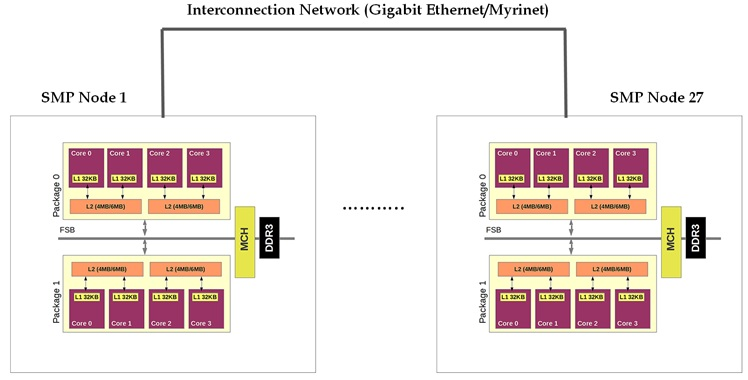
\includegraphics[width=.8\linewidth,height=\textheight,keepaspectratio]{system.jpg}
\end{figure}

\end{frame}
%------------------------------------------------
\begin{frame}
\frametitle{CGs Communication Pattern}

\begin{figure}
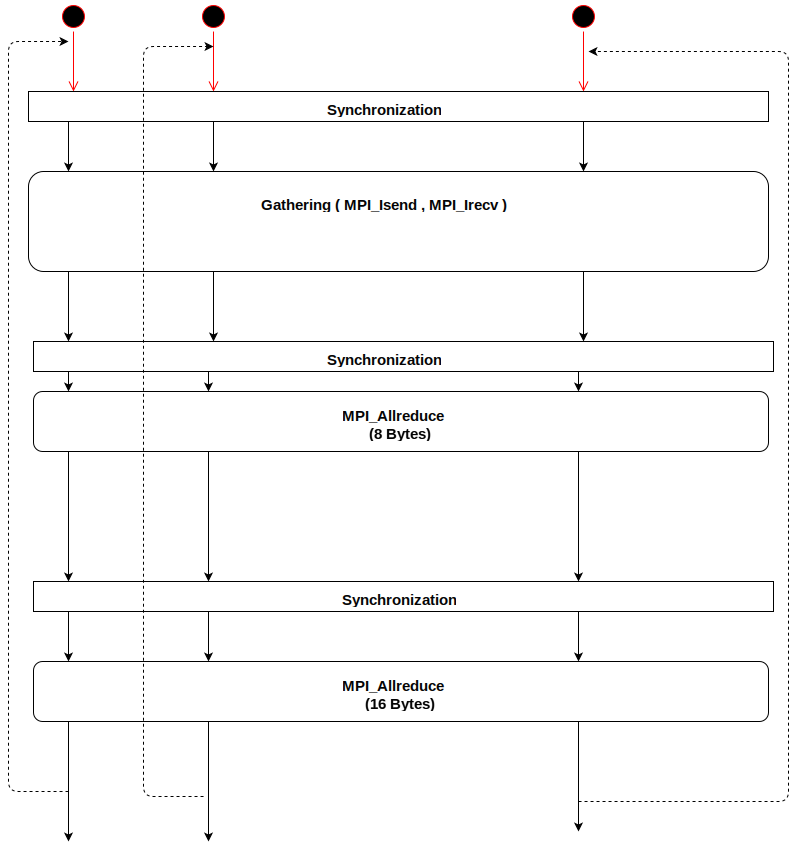
\includegraphics[height=.9\textheight, keepaspectratio]{cg.jpg}
\end{figure}

\end{frame}

%------------------------------------------------
\begin{frame}
\frametitle{Benchmarks - osu suite}
\begin{block}{P2P}
\begin{itemize}
\item \begin{alertenv}osu\_latency\end{alertenv} {\fontsize{8}{6}\selectfont ping-pong message exchange, blocking}
\item \begin{alertenv}osu\_multi\_lat \end{alertenv}{\fontsize{8}{6}\selectfont many pairs run simultaneously osu\_latency} 
\item \begin{alertenv}osu\_bw \end{alertenv}{\fontsize{8}{6}\selectfont Sender sends back to back messages and waits for ack, non blocking} 
\item \begin{alertenv}osu\_bibw \end{alertenv}{\fontsize{8}{6}\selectfont Similar with osu\_bw, both nodes send messages} 
\end{itemize}
\end{block}


\begin{block}{Collective}
\begin{alertenv}osu\_allreduce\end{alertenv}{\fontsize{8}{6} \selectfont the benchmark when run from N processes, measures the min, max and average latency of the MPI\_Allreduce operation}
\end{block}
\end{frame}
%----------------------------------------------------------------------------------------
\begin{frame}
\frametitle{Contention on Switch}

\begin{figure}
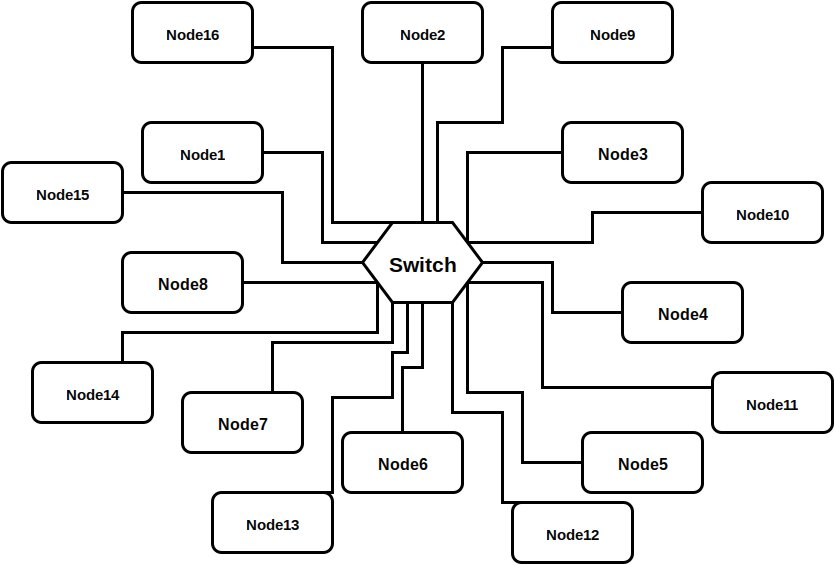
\includegraphics[width=.8\linewidth,height=\textheight,keepaspectratio]{congestion.jpg}
\caption {Systems instance for contention on switch testing}
\end{figure}

\end{frame}
%----------------------------------------------------------------------------------------
\begin{frame}
\frametitle{Contention on Switch}
\begin{columns}[c]

\column{.5\textwidth}
\begin{figure}
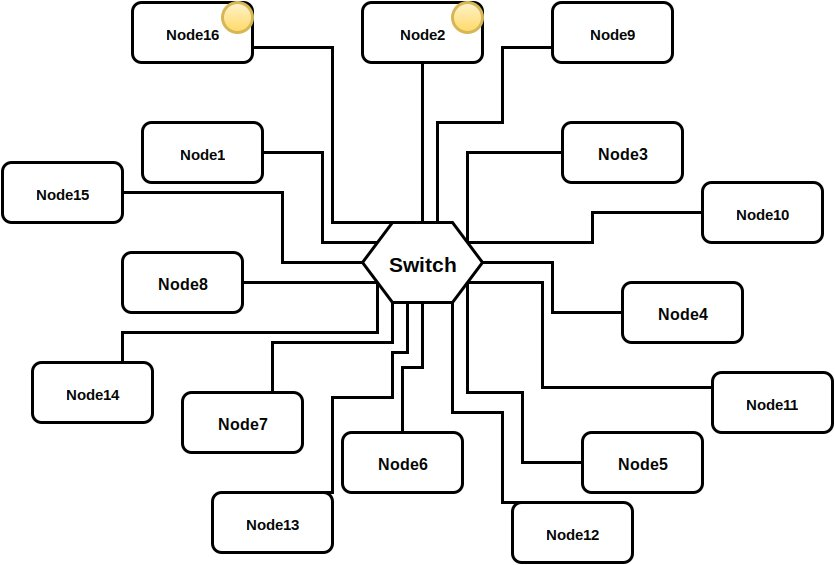
\includegraphics[width=\linewidth,height=\textheight,keepaspectratio]{congestion1.jpg}
\end{figure}

\column{.5\textwidth}
\begin{figure}
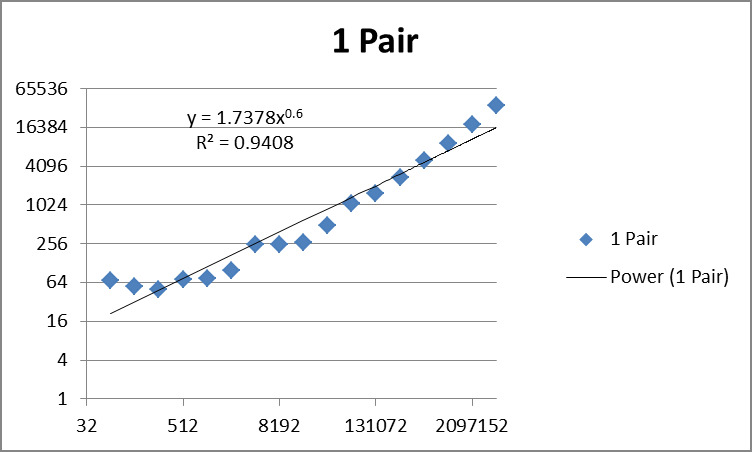
\includegraphics[width=\linewidth,height=\textheight,keepaspectratio]{picture4.jpg}
\end{figure}

\end{columns}
\begin{block}{}
\begin{equation*}
C_2 ^1(s)=\begin{cases}
50 \mu sec & \text{, if size }s < 64 \text{ Bytes} \\
1.7378\times s^{0.6} \mu sec & \text{, if size } s \geq 64 \text{ Bytes}
\end{cases}
\end{equation*}
\end{block}

\end{frame}

%----------------------------------------------------------------------------------------
\begin{frame}
\frametitle{Contention on Switch}
\begin{columns}[c]

\column{.5\textwidth}
\begin{figure}
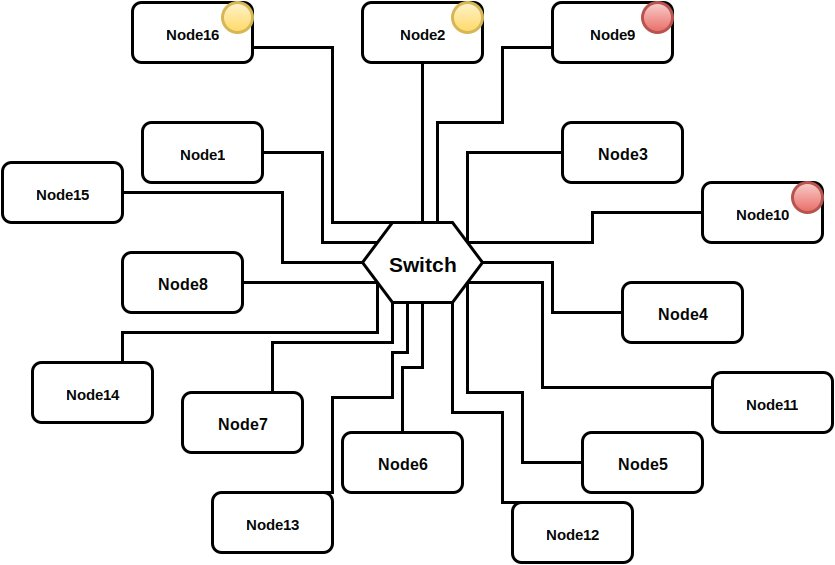
\includegraphics[width=\linewidth,height=\textheight,keepaspectratio]{congestion2.jpg}
\end{figure}

\column{.5\textwidth}
\begin{figure}
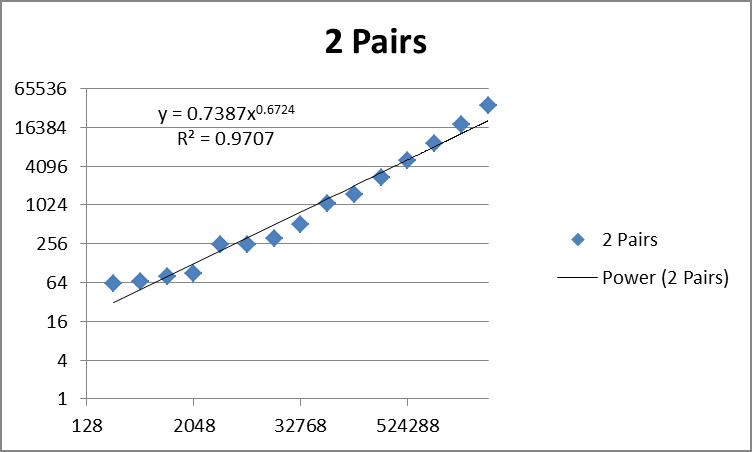
\includegraphics[width=\linewidth,height=\textheight,keepaspectratio]{picture5.jpg}
\end{figure}

\end{columns}

\begin{block}{}
\begin{equation*}
C_2 ^1(s)=\begin{cases}
50 \mu sec & \text{, if size }s < 256 \text{ Bytes} \\
0.7387\times s^{0.6724} \mu sec & \text{, if size } s \geq 256 \text{ Bytes}
\end{cases}
\end{equation*}
\end{block}

\end{frame}

%----------------------------------------------------------------------------------------
\begin{frame}
\frametitle{Contention on Switch}
\begin{columns}[c]

\column{.5\textwidth}
\begin{figure}
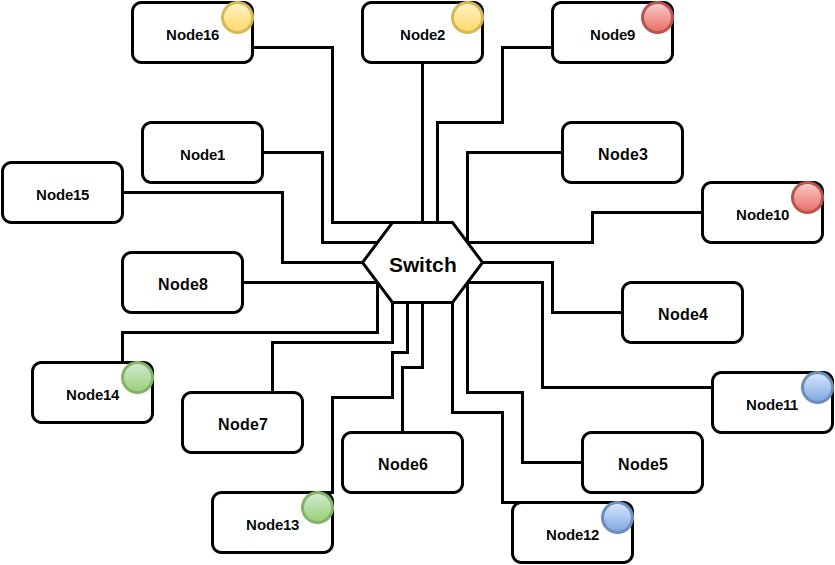
\includegraphics[width=\linewidth,height=\textheight,keepaspectratio]{congestion4.jpg}
\end{figure}

\column{.5\textwidth}
\begin{figure}
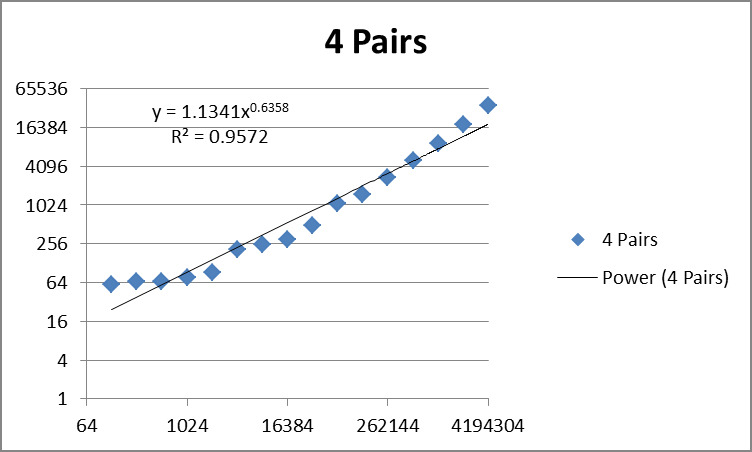
\includegraphics[width=\linewidth,height=\textheight,keepaspectratio]{picture7.jpg}
\end{figure}

\end{columns}

\begin{block}{}
\begin{equation*}
C_4 ^1(s)=\begin{cases}
50 \mu sec & \text{, if size }s < 256 \text{ Bytes} \\
1.1341\times s^{0.6358} \mu sec & \text{, if size } s \geq 256 \text{ Bytes}
\end{cases}
\end{equation*}
\end{block}

\end{frame}

%----------------------------------------------------------------------------------------
\begin{frame}
\frametitle{Contention on Switch}
\begin{columns}[c]

\column{.5\textwidth}
\begin{figure}
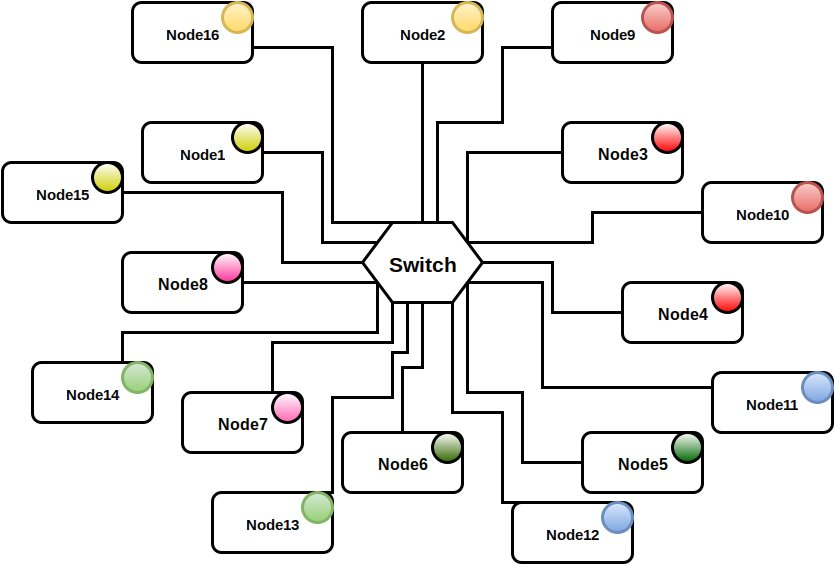
\includegraphics[width=\linewidth,height=\textheight,keepaspectratio]{congestion8.jpg}
\end{figure}

\column{.5\textwidth}
\begin{figure}
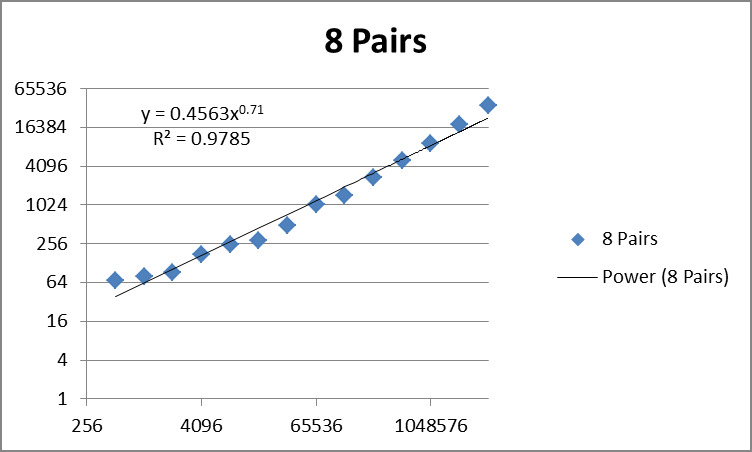
\includegraphics[width=\linewidth,height=\textheight,keepaspectratio]{picture6.jpg}
\end{figure}

\end{columns}

\begin{block}{}
\begin{equation*}
C_8 ^1(s)=\begin{cases}
50 \mu sec & \text{, if size }s < 256 \text{ Bytes} \\
0.4563\times s^{0.71} \mu sec & \text{, if size } s \geq 256 \text{ Bytes}
\end{cases}
\end{equation*}
\end{block}
\end{frame}

%----------------------------------------------------------------------------------------
\begin{frame}
\frametitle{Contention on Switch}

\begin{figure}
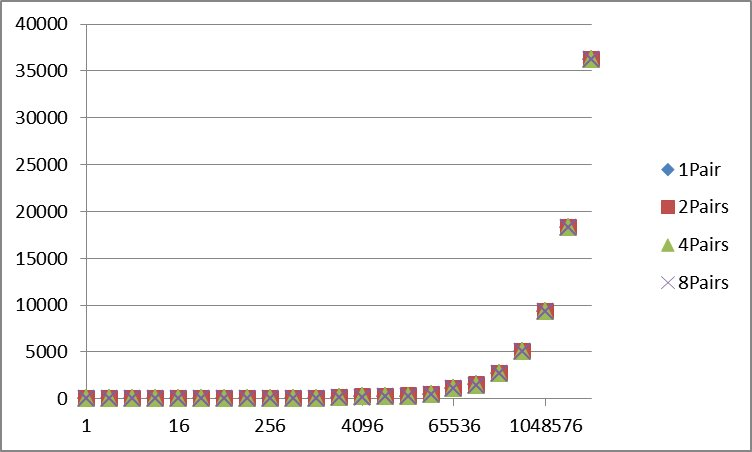
\includegraphics[width=.8\linewidth,height=\textheight,keepaspectratio]{image005.jpg}
\caption {Complete indipendancy on switch access.}
\end{figure}

\end{frame}
%----------------------------------------------------------------------------------------
\begin{frame}
\frametitle{Contention on NIC}

\begin{figure}
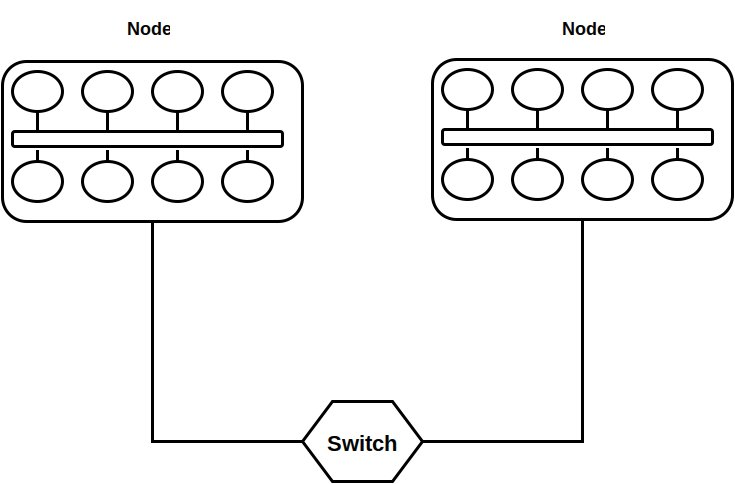
\includegraphics[width=.8\linewidth,height=\textheight,keepaspectratio]{SYSTEM.jpg}
\caption {Instance of system for contention testing}
\end{figure}

\end{frame}
%----------------------------------------------------------------------------------------
\begin{frame}
\frametitle{Contention on NIC}
\begin{columns}[c]

\column{.5\textwidth}
\begin{figure}
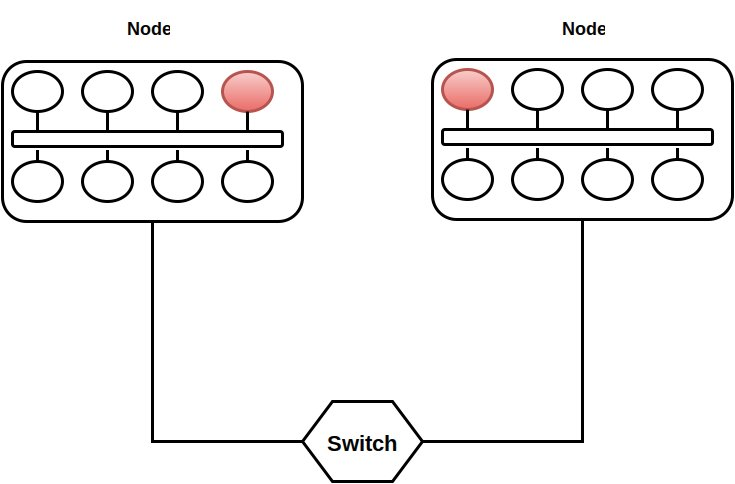
\includegraphics[width=\linewidth,height=\textheight,keepaspectratio]{nodes2p1.jpg}
\end{figure}

\column{.5\textwidth}
\begin{figure}
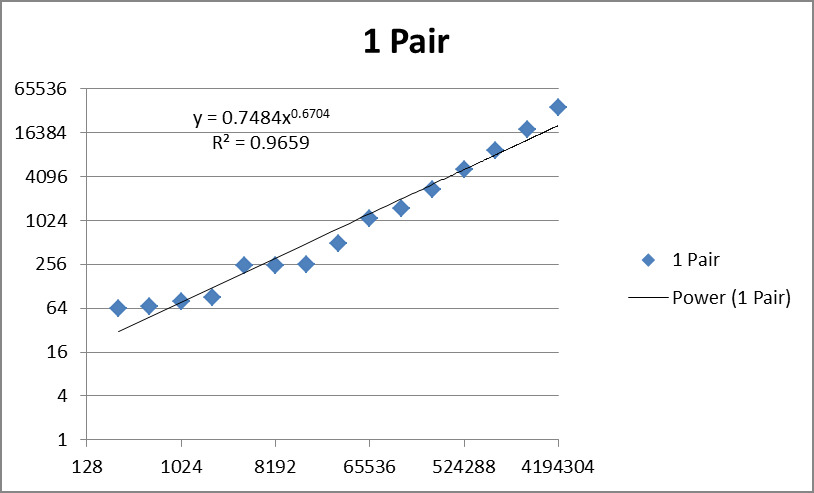
\includegraphics[width=\linewidth,height=\textheight,keepaspectratio]{picture0.jpg}
\end{figure}

\end{columns}
\begin{block}{}
\begin{equation*}
C_2 ^1 (s)=\begin{cases}
50 \mu sec & \text{, if size }s < 256 \text{ Bytes} \\
0.7484\times s^{0.6704} \mu sec & \text{, if size } s \geq 256 \text{ Bytes}
\end{cases}
\end{equation*}
\end{block}

\end{frame}

%----------------------------------------------------------------------------------------
\begin{frame}
\frametitle{Contention on NIC}
\begin{columns}[c]

\column{.5\textwidth}
\begin{figure}
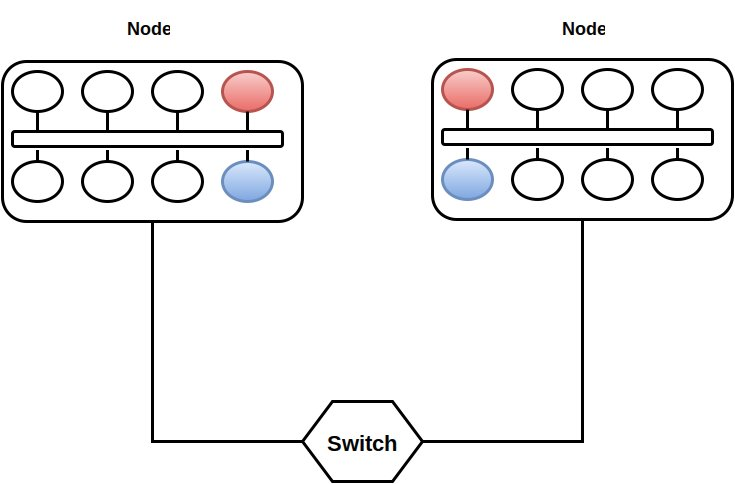
\includegraphics[width=\linewidth,height=\textheight,keepaspectratio]{nodes2p2.jpg}
\end{figure}

\column{.5\textwidth}
\begin{figure}
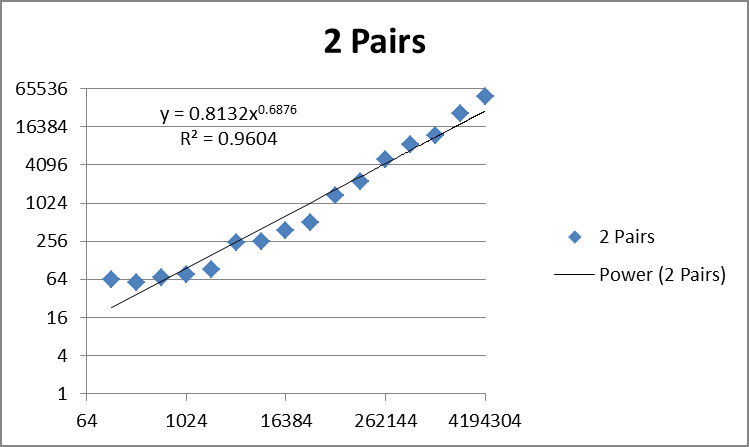
\includegraphics[width=\linewidth,height=\textheight,keepaspectratio]{picture1.jpg}
\end{figure}


\end{columns}

\begin{block}{}
\begin{equation*}
C_2 ^2(s)=\begin{cases}
50 \mu sec & \text{, if size }s < 64 \text{ Bytes} \\
0.8132\times s^{0.6876} \mu sec & \text{, if size } s \geq 64 \text{ Bytes}
\end{cases}
\end{equation*}
\end{block}

\end{frame}

%----------------------------------------------------------------------------------------

\begin{frame}
\frametitle{Contention on NIC}
\begin{columns}[c]

\column{.5\textwidth}
\begin{figure}
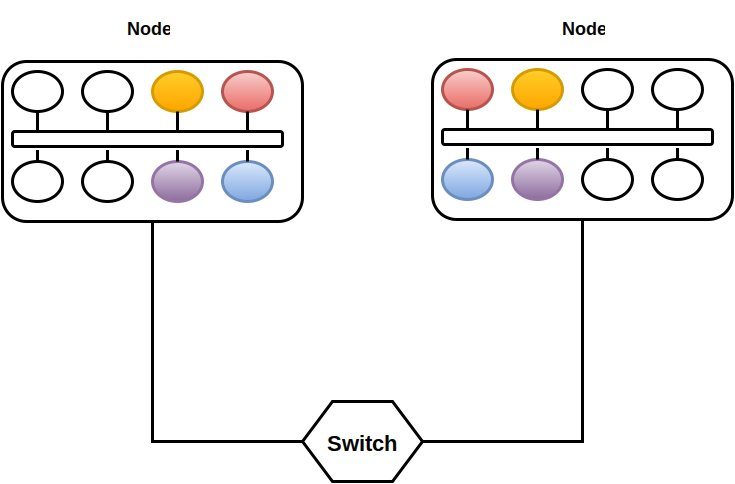
\includegraphics[width=\linewidth,height=\textheight,keepaspectratio]{nodes2p4.jpg}
\end{figure}

\column{.5\textwidth}
\begin{figure}
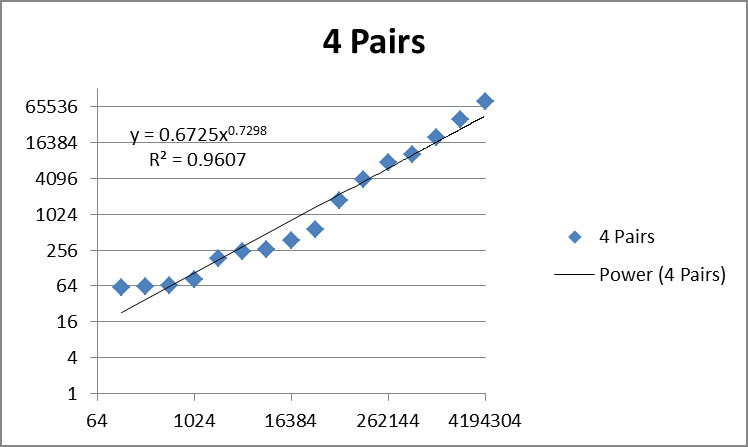
\includegraphics[width=\linewidth,height=\textheight,keepaspectratio]{picture3.jpg}
\end{figure}

\end{columns}
\begin{block}{}
\begin{equation*}
C_2 ^4 (s)=\begin{cases}
50 \mu sec & \text{, if size }s < 64 \text{ Bytes} \\
0.6725\times s^{0.7298} \mu sec & \text{, if size } s \geq 64\text{ Bytes}
\end{cases}
\end{equation*}
\end{block}

\end{frame}



%----------------------------------------------------------------------------------------

\begin{frame}
\frametitle{Contention on NIC}
\begin{columns}[c]

\column{.5\textwidth}
\begin{figure}
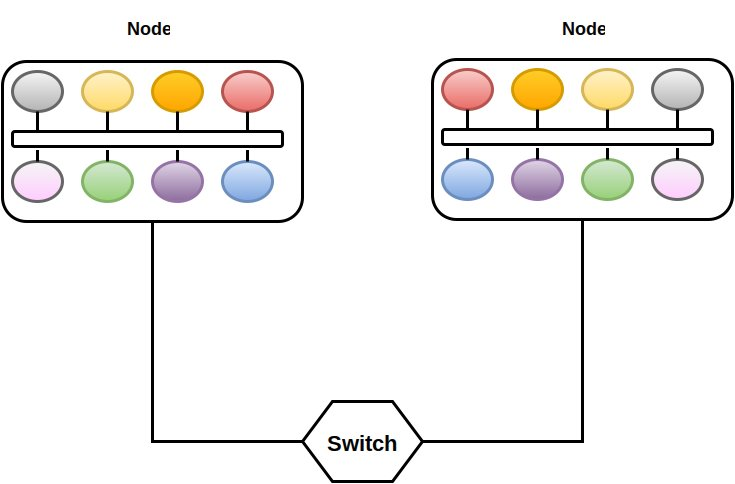
\includegraphics[width=\linewidth,height=\textheight,keepaspectratio]{nodes2p8.jpg}
\end{figure}

\column{.5\textwidth}
\begin{figure}
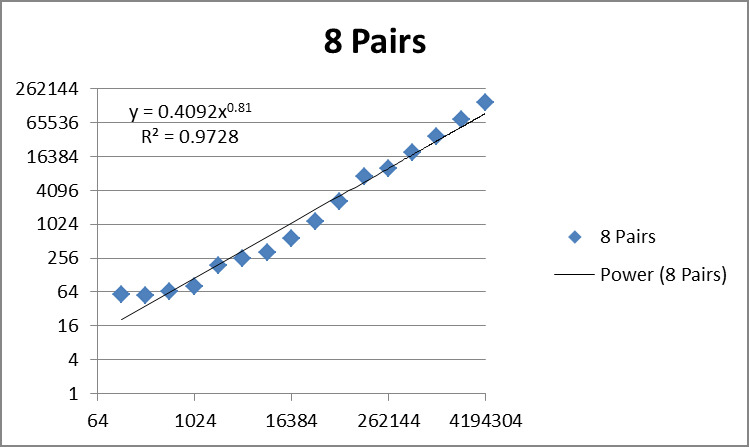
\includegraphics[width=\linewidth,height=\textheight,keepaspectratio]{picture2.jpg}
\end{figure}

\end{columns}

\begin{block}{}
\begin{equation*}
C_2 ^8(s)=\begin{cases}
50 \mu sec & \text{, if size }s < 64 \text{ Bytes} \\
0.4092\times s^{0.81} \mu sec & \text{, if size } s \geq 64 \text{ Bytes}
\end{cases}
\end{equation*}
\end{block}

\end{frame}



%-----------------------------------------------------------------------------------------
\begin{frame}
\frametitle{Contention on NIC}

\begin{figure}
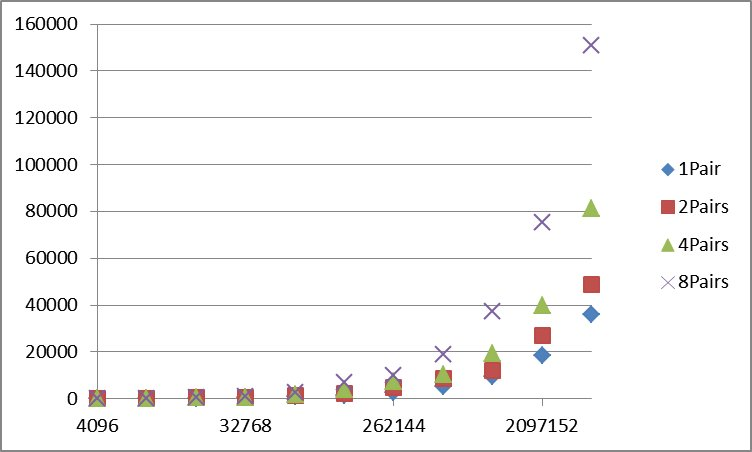
\includegraphics[width=\linewidth,height=\textheight,keepaspectratio]{image003.jpg}
\caption {Appearance of Contention on NIC}
\end{figure}

\end{frame}
%-----------------------------------------------------------------------------------------
\begin{frame}
\frametitle{Intranode Effect}

\begin{figure}
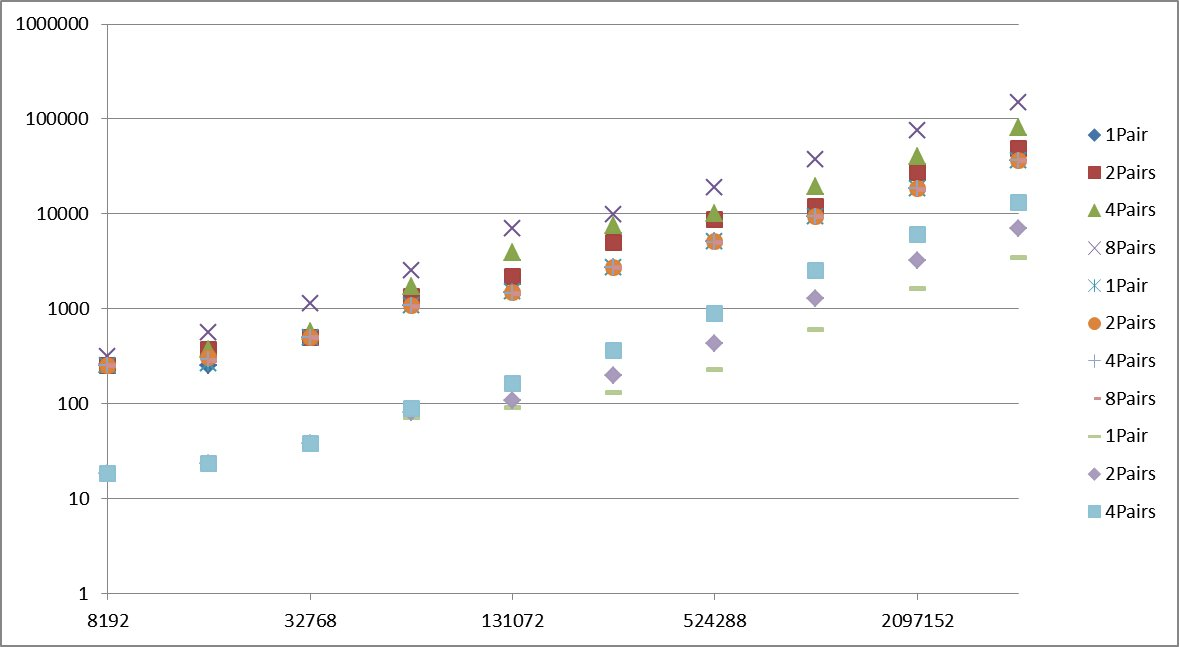
\includegraphics[width=\linewidth,height=\textheight,keepaspectratio]{image001.jpg}
\caption {Communication Overview}
\end{figure}

\end{frame}
%-----------------------------------------------------------------------------------------
%----------------------------------------------------------------------------------------
\begin{frame}
\frametitle{Useful Metrics}
\begin{itemize}
\item Maximum Send Latency
\item Maximum Receive Latency
\item Sum of Send Latencies
\item Sum of Receive Latencies
\item S+R
\end{itemize}
\end{frame}
%----------------------------------------------------------------------------------------
\begin{frame}
\frametitle{Results - Gathering Session}
\begin{columns}[c]
\column{1.1\textwidth}
\begin{table}[h!]
\centering
\caption{Prediction Results for Gathering Session}
\begin{tabular}{|c|c|c|c|}
\hline
Matrix & $S+R$ & Actual Gathering Time & Relative Deviation \\
\hline
af\_5\_k101 & 0.49985 & 0.49822 & 0.0032 \\
af\_shell10 & 0.35531 & 0.29756 & 0.1940 \\
af\_shell9 & 0.47806 & 0.40173 & 0.1900 \\
apache2 & 0.42745 & 0.35508 & 0.20381\\
bmw3\_2 & 0.34752 & 0.34752 & 0 (HIT) \\
bmwcra\_1 & 0.93015 & 0.93015 & 0 (HIT) \\
bone010 & 0.49285 & 0.49285 & 0 (HIT) \\
boneS10 & 0.42705 & 0.42705 & 0 (HIT) \\
crankseg\_2 & 0.45069 & 0.45069 & 0 (HIT) \\
F1 & 0.38515 & 0.38515 & 0 (HIT) \\
\hline
\end{tabular}
\end{table}

\end{columns}
\end{frame}
%----------------------------------------------------------------------------------------
\begin{frame}
\frametitle{Results - Gathering Session}
\begin{columns}[c]
\column{1.1\textwidth}
\begin{table}[h!]
\centering
\caption{Prediction Results for Gathering Session}
\begin{tabular}{|c|c|c|c|}
\hline
Matrix & $S+R$ & Actual Gathering Time & Relative Deviation \\
\hline
G3\_circuit & 2.44527 & 2.44527 & 0 (HIT) \\
Ga41As41H72 & 0.22786 & 0.22786 & 0 (HIT) \\
helm2d03 & 0.26700 & 0.26700 & 0 (HIT) \\
hood & 0.51297 & 0.39284 & 0.3057\\
inline\_1 & 0.89312 & 0.89312 & 0 (HIT) \\
kkt\_power & 0.42427 & 0.41462 & 0.0232\\
ldoor & 0.32107 & 0.32107 & 0 (HIT) \\
msdoor & 0.88584 & 0.88584 & 0 (HIT)\\
nd12k & 1.14328 & 1.14328 & 0 (HIT) \\
\hline
\end{tabular}
\end{table}

\end{columns}
\end{frame}
%----------------------------------------------------------------------------------------
\begin{frame}
\frametitle{Results - Gathering Session}
\begin{columns}[c]
\column{1.1\textwidth}

\begin{table}[h!]
\centering
\caption{Prediction Results for Gathering Session}
\begin{tabular}{|c|c|c|c|}
\hline
Matrix & $S+R$ & Actual Gathering Time & Relative Deviation \\
\hline
nd24k & 0.72550 & 0.72550 & 0 (HIT) \\
nd6k & 0.24027 & 0.22966 & 0.0461 \\
parabolic\_fem & 0.23146 & 0.23146 & 0 (HIT) \\
pwtk & 0.28839 & 0.24462 & 0.1789\\
s3dkq4m2 & 0.19154 & 0.19154 & 0 (HIT) \\
ship\_001 & 2.13303& 2.13303 & 0 (HIT) \\
Si41Ge41H72 & 2.48232 & 2.48232 & 0 (HIT) \\
Si87H76 & 0.23744 & 0.23744 & 0 (HIT) \\
thermal2 & 0.47869 & 0.47869 & 0 (HIT) \\
thread & 0.31130 & 0.31130 & 0 (HIT) \\
\hline
\end{tabular}
\end{table}

\end{columns}
\end{frame}
%----------------------------------------------------------------------------------------
\begin{frame}
\frametitle{Collective Communication}

\begin{table}[h]
\centering
\caption{Collective Communication Latency, Message size $<$ 64B }
\begin{tabular}{|c|c|c|}
\hline
\multicolumn{3}{|c|}{Latency($\mu$sec), 2 Nodes}\\
\hline
2 Pairs & 4 Pairs & 8 Pairs\\
\hline
84.79 & 121.48 & 171.23\\
\hline
\end{tabular}
\end{table}




\begin{table}[h]
\centering
\caption{Collective Communication Latency, Message size $<$ 64B }
\begin{tabular}{|c|c|c|c|}
\hline
\multicolumn{4}{|c|}{Latency($\mu$sec), 4 Nodes}\\
\hline
2 Pairs & 4 Pairs & 8 Pairs & 16 Pairs\\
\hline
120.22 & 144.21 & 185.33 & 255.66 \\
\hline
\end{tabular}
\end{table}




\begin{table}[h]
\centering
\caption{Collective Communication Latency, Message size $<$ 64B }
\begin{tabular}{|c|c|c|c|c|}
\hline
\multicolumn{5}{|c|}{Latency($\mu$sec), 8 Nodes}\\
\hline
2 Pairs & 4 Pairs & 8 Pairs & 16 Pairs & 32 Pairs\\
\hline
104.01 & 191.17 & 219.28 & 242.27 & 346.17 \\
\hline
\end{tabular}
\end{table}

\end{frame}


\begin{frame}
\frametitle{Collective Communication Predictor}

\begin{table}[h]
\centering
\caption{Collective Communication Predictor for CG}
\begin{tabular}{|c|c|c|c|}
\hline
& \multicolumn{3}{|c|}{Latency($\mu$sec)}\\
\hline
Processes Per Node & 2 Nodes & 4 Nodes& 8 Nodes\\
\hline
4 PPN & 242.96 & 370.66  & 484.54\\
8 PPN & 342.46 & 511.32 & 692.34\\ 
\hline
\end{tabular}
\end{table}
\end{frame}
%----------------------------------------------------------------------------------------

\begin{frame}
\frametitle{Results - Entire Communication}
\begin{columns}[c]
\column{1.1\textwidth}

\begin{table}[h!]
\centering
\caption{Prediction Results for CG}
\begin{tabular}{|c|c|c|c|}
\hline
 & & Actual& \\
Matrix & $S+R+A$ &Communication Time & Relative Deviation \\
\hline
af\_5\_k101 & 0.92685 & 0.92685 & 0 (HIT) \\
af\_shell10 & 0.75131 & 0.72214 & 0.0011 \\
af\_shell9 & 0.87909 & 0.87909 & 0 (HIT) \\
apache2 & 0.81645 & 0.72729 & 0.1225\\
bmw3\_2 & 0.77252 & 0.77252 & 0 (HIT) \\
bmwcra\_1 & 1.34415 & 1.34415 & 0 (HIT) \\
bone010 & 0.90385 & 0.90385 & 0 (HIT) \\
boneS10 & 0.82305 & 0.82305 & 0 (HIT) \\
crankseg\_2 & 0.84369 & 0.84369 & 0 (HIT) \\
F1 & 0.82350 & 0.78090 & 0.0545 \\
\hline
\end{tabular}
\end{table}
\end{columns}
\end{frame}

%----------------------------------------------------------------------------------------
\begin{frame}
\frametitle{Results - Entire Communication}
\begin{columns}[c]
\column{1.1\textwidth}

\begin{table}[h!]
\centering
\caption{Prediction Results for CG}
\begin{tabular}{|c|c|c|c|}
\hline
 & & Actual& \\
Matrix & $S+R+A$ &Communication Time & Relative Deviation \\
\hline
G3\_circuit & 2.84727 & 2.84727 & 0 (HIT) \\
Ga41As41H72 & 0.61586 & 0.61586 & 0 (HIT) \\
helm2d03 & 0.66215 & 0.66215 & 0 (HIT) \\
hood & 1.13997 & 0.79384 & 0.4360 \\
inline\_1 & 1.33412 & 1.33412 & 0 (HIT) \\
kkt\_power & 0.84827 & 0.77354 & 0.0966 \\
ldoor & 0.71707 & 0.69761 & 0.0278 \\
msdoor & 1.28484 & 1.28484 & 0 (HIT) \\
nd12k & 1.55428 & 1.55428 & 0 (HIT) \\
\hline
\end{tabular}
\end{table}
\end{columns}
\end{frame}

%----------------------------------------------------------------------------------------
\begin{frame}
\frametitle{Results - Entire Communication}
\begin{columns}[c]
\column{1.1\textwidth}

\begin{table}[h!]
\centering
\caption{Prediction Results for CG}
\begin{tabular}{|c|c|c|c|}
\hline
 & & Actual& \\
Matrix & $S+R+A$ &Communication Time & Relative Deviation \\
\hline
nd24k & 1.11750 & 1.01191 & 0.1043 \\
nd6k & 0.50727 & 0.50727 & 0 (HIT) \\
parabolic\_fem & 0.62846 & 0.62846 & 0 (HIT) \\
pwtk & 0.67739 & 0.67739 & 0 (HIT) \\
s3dkq4m2 & 0.58054 & 0.58054 & 0 (HIT) \\
ship\_001 & 2.52803 & 2.52803 & 0 (HIT) \\
Si41Ge41H72 & 2.87932 & 2.87932 & 0 (HIT) \\
Si87H76 & 0.65244 & 0.65244 & 0 (HIT) \\
thermal2 & 0.86769 & 0.86769 & 0 (HIT) \\
thread & 0.72289 & 0.72289 & 0 (HIT) \\
\hline
\end{tabular}
\end{table}
\end{columns}
\end{frame}

%----------------------------------------------------------------------------------------
\begin{frame}
\frametitle{Results}

\begin{columns}[c]

\column{.5\textwidth}
\begin{block}{Accuracy on Gathering Session}
$$\frac{hit}{miss}=\frac{21}{8}$$
$$ \text{Deviation}_{S+R}=4.05\%$$
\end{block}
\column{.5\textwidth}
\begin{block}{Accuracy on the entire communication pattern}
$$\frac{hit}{miss}=\frac{22}{7}$$
$$ \text{Deviation}_{S+R+A}=2.91\%$$
\end{block}
\end{columns}

\end{frame}
%----------------------------------------------------------------------------------------
\begin{frame}
\frametitle{Conclusions}

\begin{itemize}
\item {\fontsize{8}{6}\selectfont We attempted to predict the optimal placement for CG }
\item {\fontsize{8}{6}\selectfont We performed a series of benchmarks in order to explore systems behavior}
\item {\fontsize{8}{6}\selectfont We finally predicted the optimal placement for both the dominant session as well as the entire communication of CG, with satisfying accuracy and deviation.}
\end{itemize}

\end{frame}

\end{document} 
%----------------------------------------------------------------------------------------
